```latex
\documentclass[12pt,a4paper]{article}
\usepackage[utf8]{inputenc}
\usepackage{xcolor}
\usepackage{tikz}
\usepackage[margin=1in]{geometry}

\newcommand{\bitstuff}[1]{\textcolor{red}{\textbf{#1}}}
\newcommand{\flag}[1]{\textcolor{blue}{\textbf{#1}}}

\begin{document}

\begin{center}
\textbf{Computer Networks: Bit Stuffing with FLAGS}
\end{center}

\textbf{Original Data:} \texttt{0101011111101000000101111101}

\textbf{Bit Stuffing Process:}

1. \textbf{Data from Upper Layer:}
   \begin{center}
   \fbox{\texttt{0101011111101000000101111101}}
   \end{center}

2. \textbf{Stuffed Data (Sender's End):}
   \begin{center}
   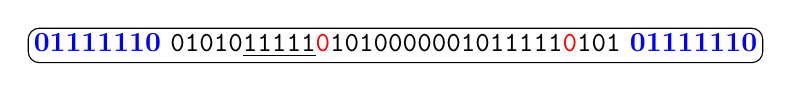
\begin{tikzpicture}
   \node[draw,rounded corners,inner sep=2pt] {
   \flag{01111110} \texttt{01010\underline{11111}\bitstuff{0}1010000001011111\bitstuff{0}101} \flag{01111110}
   };
   \end{tikzpicture}
   \end{center}

3. \textbf{Frame Sent:}
   \begin{center}
   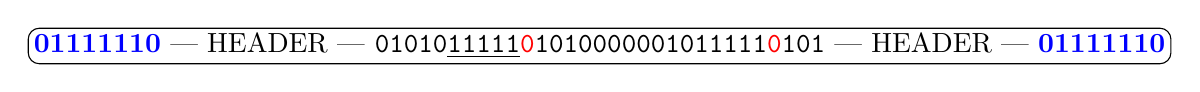
\begin{tikzpicture}
   \node[draw,rounded corners,inner sep=2pt] {
   \flag{01111110} | HEADER | \texttt{01010\underline{11111}\bitstuff{0}1010000001011111\bitstuff{0}101} | HEADER | \flag{01111110}
   };
   \end{tikzpicture}
   \end{center}

4. \textbf{Frame Received (Receiver's End):}
   \begin{center}
   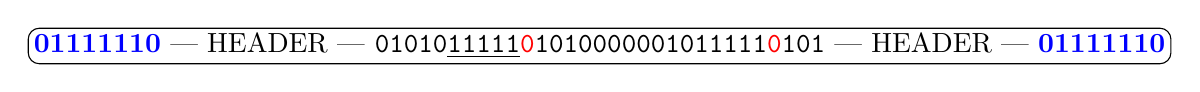
\begin{tikzpicture}
   \node[draw,rounded corners,inner sep=2pt] {
   \flag{01111110} | HEADER | \texttt{01010\underline{11111}\bitstuff{0}1010000001011111\bitstuff{0}101} | HEADER | \flag{01111110}
   };
   \end{tikzpicture}
   \end{center}

5. \textbf{Un-Stuffed Data:}
   \begin{center}
   \fbox{\texttt{0101011111101000000101111101}}
   \end{center}

\textbf{Explanation:}
- FLAG (\flag{01111110}) is added at the beginning and end of the frame.
- \bitstuff{0} (in red) are the stuffed bits, inserted after every five consecutive 1's.
- The stuffing process ensures that the bit pattern of the FLAG doesn't appear in the data.
- At the receiver's end, stuffed 0's are removed to recover the original data.

\end{document}
```